\section{Dynamic Simulation of the Arm: A Comprehensive Model for Musculoskeletal Dynamics}
The study of human mobility has benefited greatly from the development of musculoskeletal modeling, which is now a crucial tool for comprehending the dynamics of the human body. Multibody models have historically proved helpful in resolving inverse dynamic issues, particularly in the analysis of human gait and arm movement (please add paper citation for more information). The main disadvantage of these inverse dynamic techniques is the need to gather data from participants who are actively doing the required movement.

Moving away from conventional techniques, muscle-driven forward dynamics have allowed the simulation of innovative and fictional movements that would resemble impaired movements, such as those of stroke survivors. These simulations have practical applications in fields like rehabilitation and motor control research. In \cite{IMP} the DAS allowed to test controllers and command interfaces with a human user in the loop. For this project, forward dynamics simulation will be used to test the hypothesis for EMG-inspired PD control of Functional Electrical Stimulation (FES) in stroke rehabilitation. 

A summary of the musculoskeletal dynamics, including topics like multibody dynamics, muscle contraction dynamics, and muscle activation dynamics, will be covered in this section. Then, an explanation of the forward-dynamic implicit formulation will be given. This formulation is proven to improve the computational time required for modeling the dynamics with only an RMS error of 0.11 degrees in joint angles when running at real-time speed for a gait simulation with a prosthetic foot and ankle \cite{IMP}.

Overall, the Dynamic Arm Simulator (DAS) offers a robust framework for the simulation of human arm movements. It is implemented as a MATLAB Mex function that contains the system dynamics and other functions, making it accessible via a MATLAB function interface and flexible and adaptable for various applications. 

An extended overview of the DAS model follows in the sections below.

\subsection{Structural Overview}
Links and Degrees of Freedom
\begin{itemize}
    \item \textbf{7 Links}: Includes thorax, clavicle, scapula, humerus, ulna, radius, and hand. Figure \ref{fig:links} shows a colour-coded of the different links. 
\end{itemize}
\begin{figure}[h!]
    \centering
    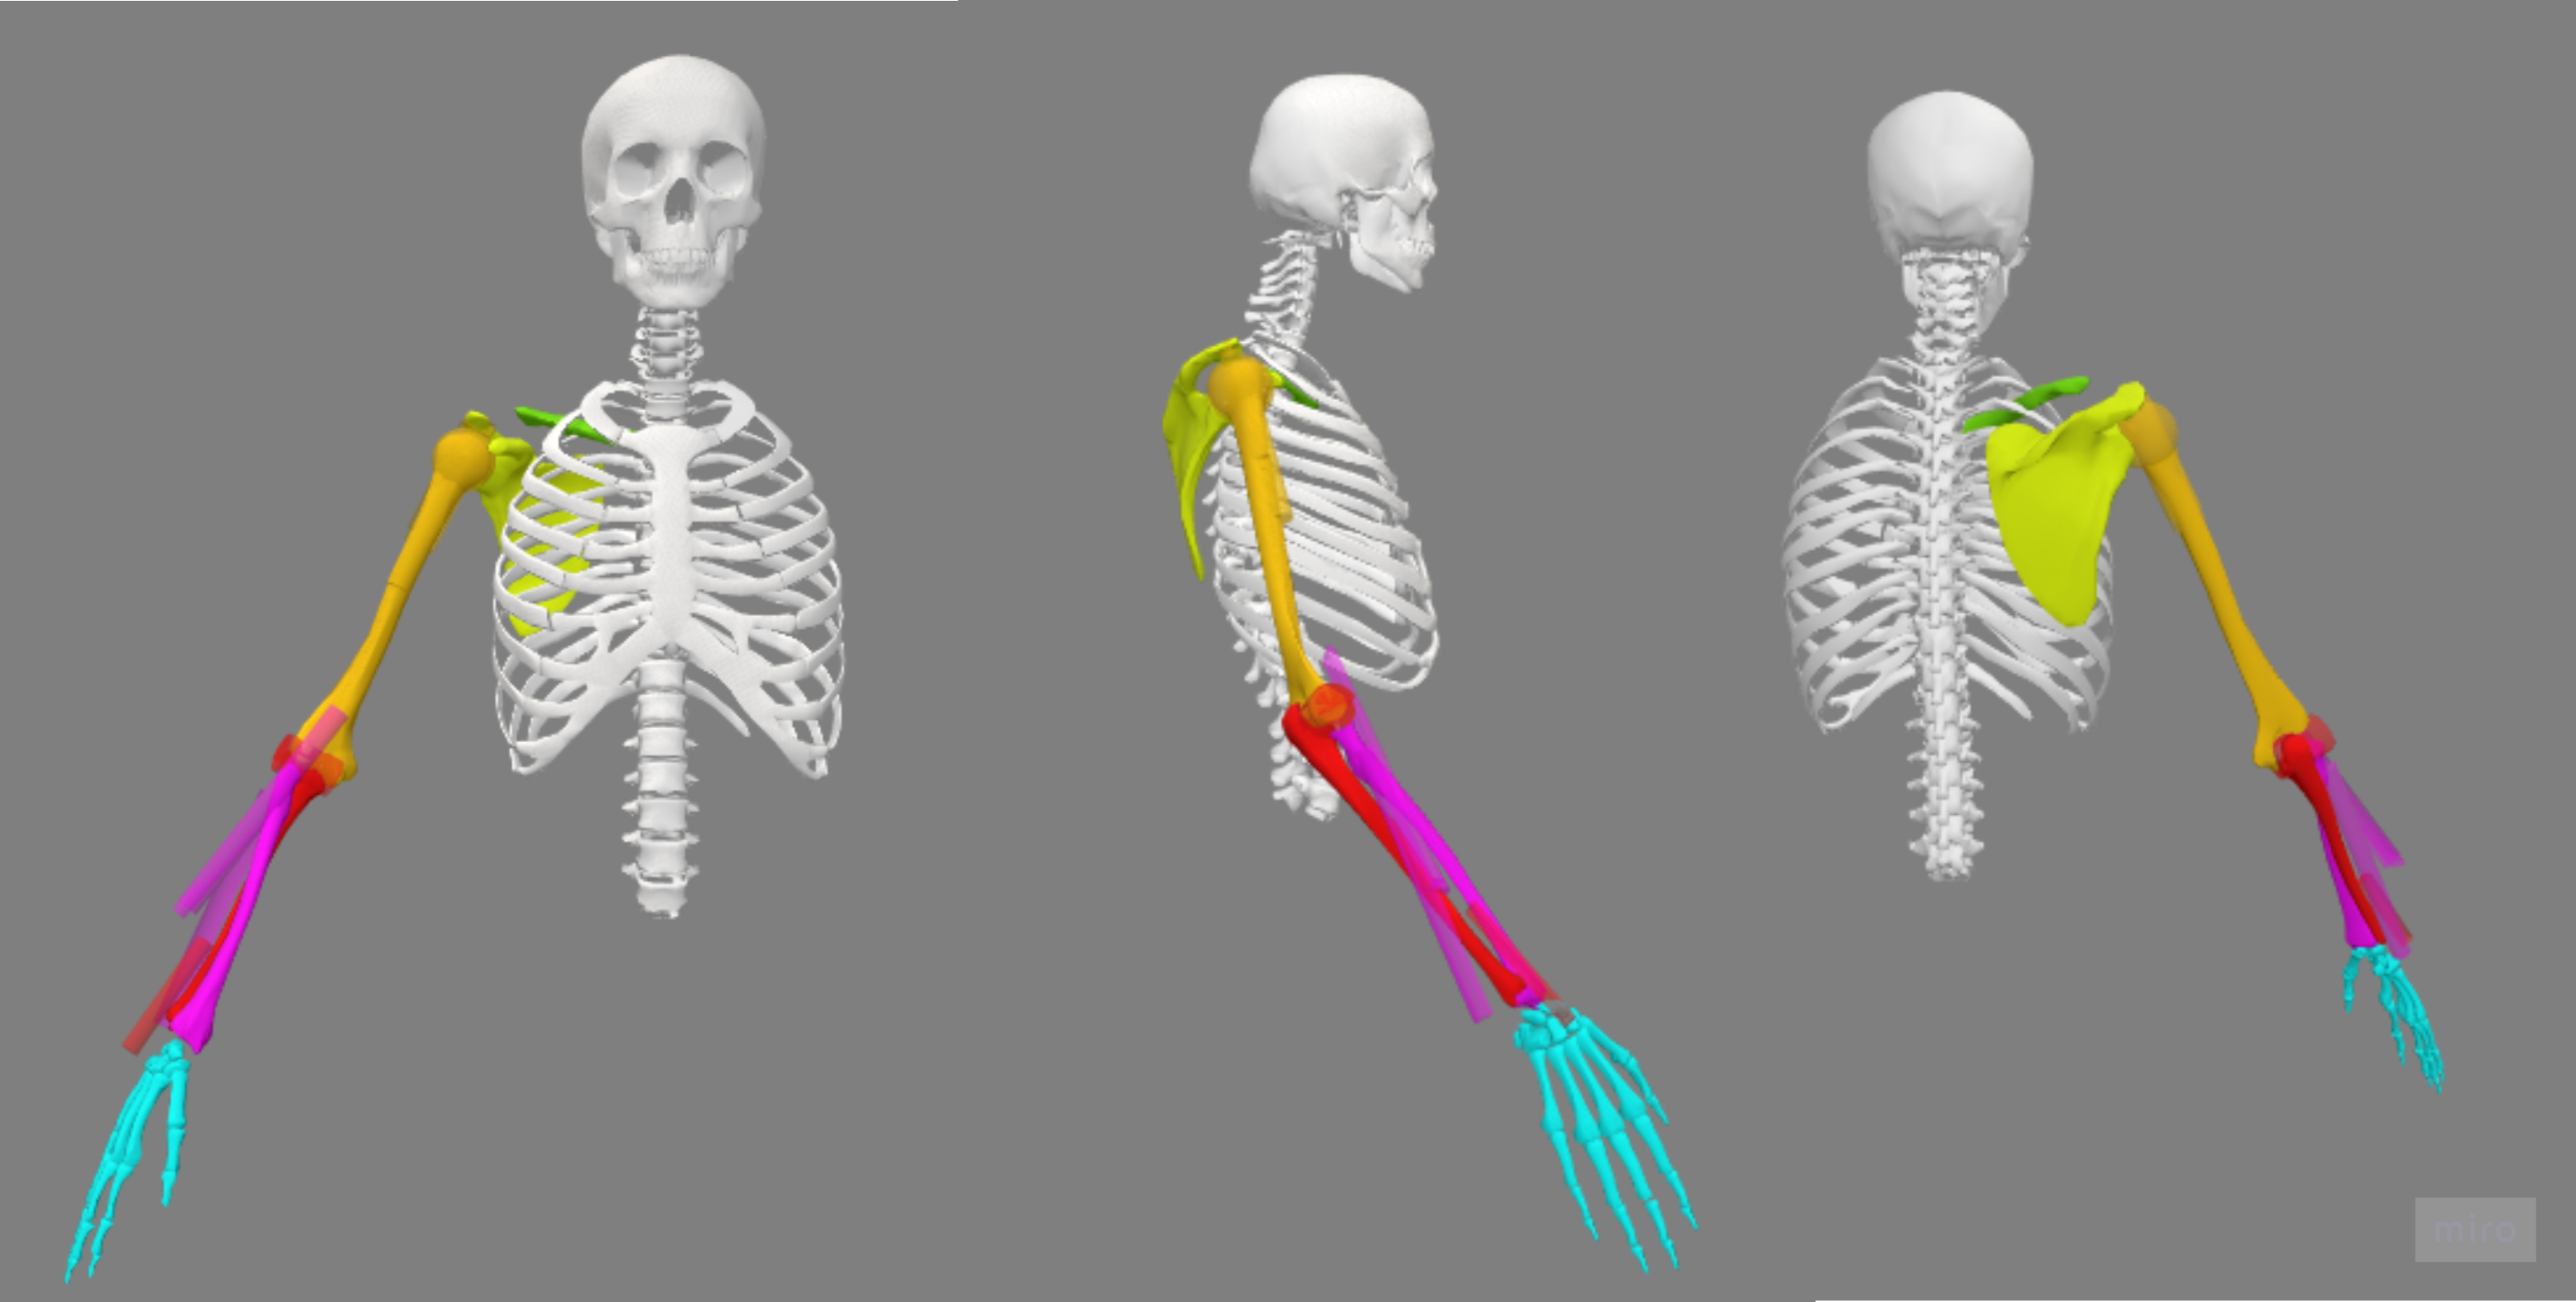
\includegraphics[width=0.7\textwidth]{Pictures/DAS/Links.png}
    \caption{Dynamic Arm Simulator 7 Links. Green: Clavicle, Yellow: Scapula, Orange: humerus, Red: Ulna, Purple: Radius, Blue: hand}
    \label{fig:links}
\end{figure}

\begin{itemize}
    \item \textbf{11 Degrees of Freedom}: These are comprised of 2 orthogonal hinges at specific joints including the sterno-clavicular, acromio-clavicular, and Gh joints, elbow flexion-extension, and forearm pronation-supination. The range of motion of the different DoF is shown in Table \ref{table:11dof}.\newline
    Inspired on \cite{RT3D} throughout this project the arm configuration is described in 5 DoF: plane of elevation, angle of elevation, internal rotation, elbow flexion and forearm pronation following the recommendation on \cite{ISB}. These angles were restricted in order to ensure correct wrapping of muscles in the model, the final values are show in Figure \ref{fig:5dof}.
\end{itemize}

\begin{table}[h!]
\centering
\caption {\textit{Angular limits for each degree of freedom (in degrees)}: The arm mechanism consists of the following skeletal entities SC: Sternoclavicular joint, AC: Acromioclavicular joint, Gh: Glenohumeral joint, EL: Elbow, PS: Forearm Pronation and Supination.}
\label{table:11dof}
\begin{tabular}{ccc}
\hline
\textbf{Degree of Freedom} & \textbf{Min Angle (degrees)} & \textbf{Max Angle (degrees)} \\
\hline
SC y & -65.00 & -19.00 \\
SC z & 5.00 & 30.00 \\
SC x & 0.00 & 83.00 \\
AC y & 33.00 & 69.00 \\
AC z & -22.00 & 20.00 \\
AC x & -17.00 & 18.00 \\
Gh y & -170.00 & 175.00 \\
Gh z & -30.00 & 84.00 \\
Gh yy & -177.00 & 179.00 \\
EL x & 5.00 & 141.00 \\
PS y & 5.00 & 160.00 \\
\hline
\end{tabular}

\end{table}

\begin{figure}[h!]
    \centering
    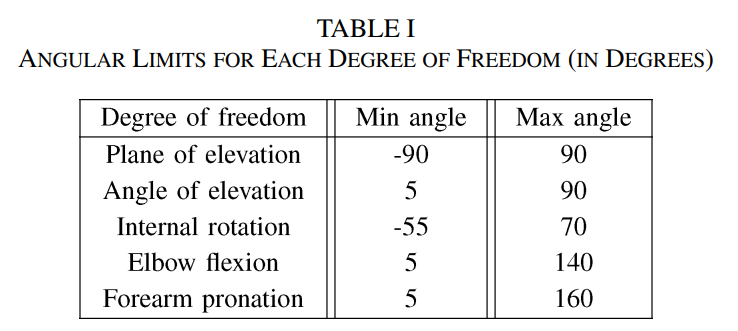
\includegraphics[width=0.7\textwidth]{Pictures/DAS/5dof.png}
    \caption{Angular limits for each degree of freedom (in degrees) for the arm configuration following \cite{ISB}. Table from \cite{RT3D}}
    \label{fig:5dof}
\end{figure}
\newpage
\begin{itemize}
    \item \textbf{22 Muscles and 138 Muscle Elements:} The real-time model consists of 22 muscles and muscle components in total. In order to accurately represent the mechanical line of action of each member, muscles are modeled using the fewest amount of parts possible. The table in Figure  \ref{fig:muscle_elements} displays the amount of elements utilized for each muscle as well as the degrees of freedom that each muscle crosses 
    
\end{itemize}

\begin{figure}[ht!]
    \centering
    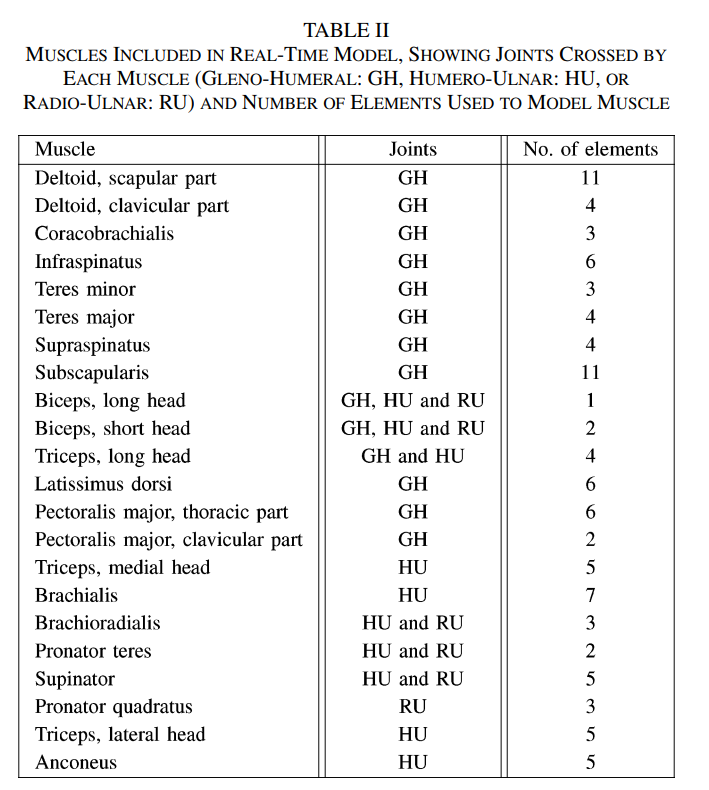
\includegraphics[width=0.7\textwidth]{Pictures/DAS/muscles_elements.png}
    \caption{Muscle elements and degrees of freedom crossed by the muscles. Table from \cite{RT3D}}
    \label{fig:muscle_elements}
\end{figure}


\subsection{Musculoskeletal Dynamics}
% To do:: Explain the state variable and create a nomenclature table
The dynamics governing the musculoskeletal system must be thoroughly understood in order to research it. This analysis is divided into three interconnected components: multibody dynamics, muscle activation dynamics, and muscle contraction dynamics. Multibody dynamics allows us to represent the system as a collection of interconnected rigid or flexible bodies, focusing on the kinematic constraints that guide motion. Muscle contraction dynamics describes the complex interactions of the muscle fibers and surrounding elements using the three-element Hill-type model, while muscle activation dynamics explores how neural signals translate into muscle actions.

The thorough analysis of the musculoskeletal dynamics is described in \cite{IMP}. In this section a summary of each most relevant section is presents with specific focus on the project's application.
\newline

\subsubsection{State variables}

It is necessary to define the state variables before examining the various dynamics of the multibody system.

The multibody model has 298 state variables. It is represented with the letter\textbf{ \textit{x}}:
\begin{itemize}
    \item 11 angles, $q$
    \item 11 angular velocities, $\dot{q}$
    \item 138 muscle contractile element (CE) lengths, $L_{CE}$
    \item 138 muscle active states, $a$
\end{itemize}

 
\subsubsection{Multibody dynamics}

Multibody dynamics is used to study the motion and forces acting on the musculoskeletal system as it is identified as a system composed of interconnected rigid or flexible bodies. 

Generalized coordinates are used to simplify the description of the system. As a result, the configuration of the system can be represented using the minimum number of coordinates to described the position and orientation.  

Generalized coordinates, are often denoted by \textit{q}. They are set of independent parameters that define the configuration of the system. In the DAS \textit{q} represents the 11 joint angles. 

The equations of motion for a multibody system can be expressed in the following matrix form (\cite{Siciliano2009}):
\begin{equation}
    M(q)*\Ddot{q} + B(q,\dot{q}) = \tau
    \label{eq:MBD}
\end{equation}

Where,
\begin{itemize}
    \item $\ddot{q}$ is the vector of generalized accelerations
    \item $M(q)$ is the mass matrix that describes the inertia of the system. It relates the acceleration of \textit{q} to the generalized forces.
    \item $B(q,\dot{q})$ is the matrix that described Coriolis and centrifugal forces that arise from the motion of the bodies in the system. Moreover, it contains gravity and other passive forces.
    \item $\tau$ is the generalized forces vector. In the case of DAS it represents the forces generated by muscles according to the muscle contraction and activation dynamics. 
\end{itemize}

Forward dynamics is used to predict the motion of a multibody system based on its initial conditions and known forces. As a result Equation \ref{eq:MBD} is solved to the generalized accelerations $\ddot{q}$.

\begin{equation}
    \ddot{q} = M(q)^{-1}(\tau - B(q,\dot{q}))
\end{equation}

The inverse of the mass matrix, $M$, is a critical component, as the simulation will not be possible if its singular. This singularity is quite common in musculoskeletal systems due to small mass and moment of inertia of body segments.

Moreover, elements of $B$ can present high stiffness and damping, leading to high eigenvalues of the Jacobian matrix that correspond to fast-changing components of the system. These high stiffness and high damping lead to oscillatory behaviours within the system. The presence of stiffness, originates from the ligaments and tendons having highly nonlinear mechanical properties (zero stiffness when unloaded, high stiffness when maximally loaded).

To counteract the stiff system, standard numerical methods, such as Euler method, require small time steps.


\newline \newline
\subsubsection{Muscle contraction dynamics}

The muscle contraction dynamics is based on the three-element Hill-type model. It represents the muscle fibers (CE: contractile element), the tendon and force transmitting tissue (SEE: series elastic element), and the passive elastic tissue surrounding the muscle fibers (PEE: passive elastic element). 
\begin{figure}[ht!]
    \centering
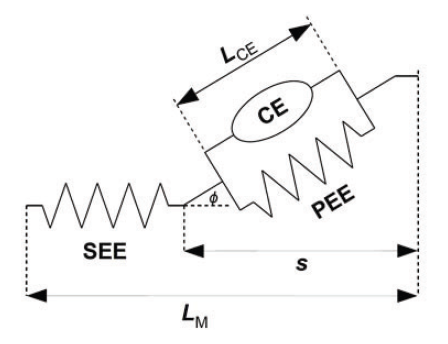
\includegraphics[width=0.4\textwidth]{Pictures/DAS/Hill-Type_MuscleModel.png}
    \caption{Three-element muscle model. CE: contractile element, SEE: series elastic element, PEE: parallel elastic element, Pennation angle $\phi$: Angle between the muscle fiber in the CE and the line of action of the muscle, $s$ state variable for the muscle contraction dynamics \cite{IMP}}
    \label{fig:muscle_elements}
\end{figure}

The contractile force is calculated by the multiplicative interaction of the maximal isometric force, the activation, the fiber length and the fiber length velocity, respectively represented in the formula below:
\begin{equation}
    F_{CE} = F_{max}*a*f_{FL}(L_{CE})*f_{FV}(\dot{L_{CE}})
\end{equation}

The series and parallel elastic elements are represented by passive force-length relationships.
\begin{equation}
    F_{SEE} = f_{SEE}(L_{M}-L_{CE}*cos(\phi))
\end{equation}
\begin{equation}
    F_{PEE} = f_{PEE}(L_{CE})
\end{equation}

The force balance equation following Figure \ref{fig:muscle_elements} is equal to:
\begin{equation}
    (F_{CE}+F_{PEE})*cos(\phi) - F_{SEE} = 0
    \label{eq:MCD}
\end{equation}

The differential equation for the state variable $L_{CE}$ is defined by Equation \ref{eq:MCD}.  
\newline
\subsubsection{Muscle activation dynamics}

The nervous system sends a neural excitation $u(t)$ as a control signal into the muscle that changes the activation via  a first-order nonlinear activation-deactivation process. This is because the activation $a$, also called \textit{active state} cannot be directly controlled by the nervous system. The  muscle activation of a muscle, $a$, is formulated as:

\begin{equation}
    \dot{a} = (u-a)(c_{1}u + c_{2})
    \label{eq:MAD}
\end{equation},

where $c_{1} + c_{2}$ is the rate constant for activation and $c_{2}$ is the rate constant for deactivation, typically in the range of 20-50 $s^{-1}$ \cite{IMP}.

Combining Equation \ref{eq:MBD}, Equation \ref{eq:MCD} and Equation \ref{eq:MAD} an implicit state equation for musculoskeletal dynamics can be formulated.  

\subsection{Forward Dynamics for implicit state equation}
\subsection{Functionalities}